\documentclass{standalone}
\usepackage{pgfplots}
\pgfplotsset{compat=newest}

\begin{document}
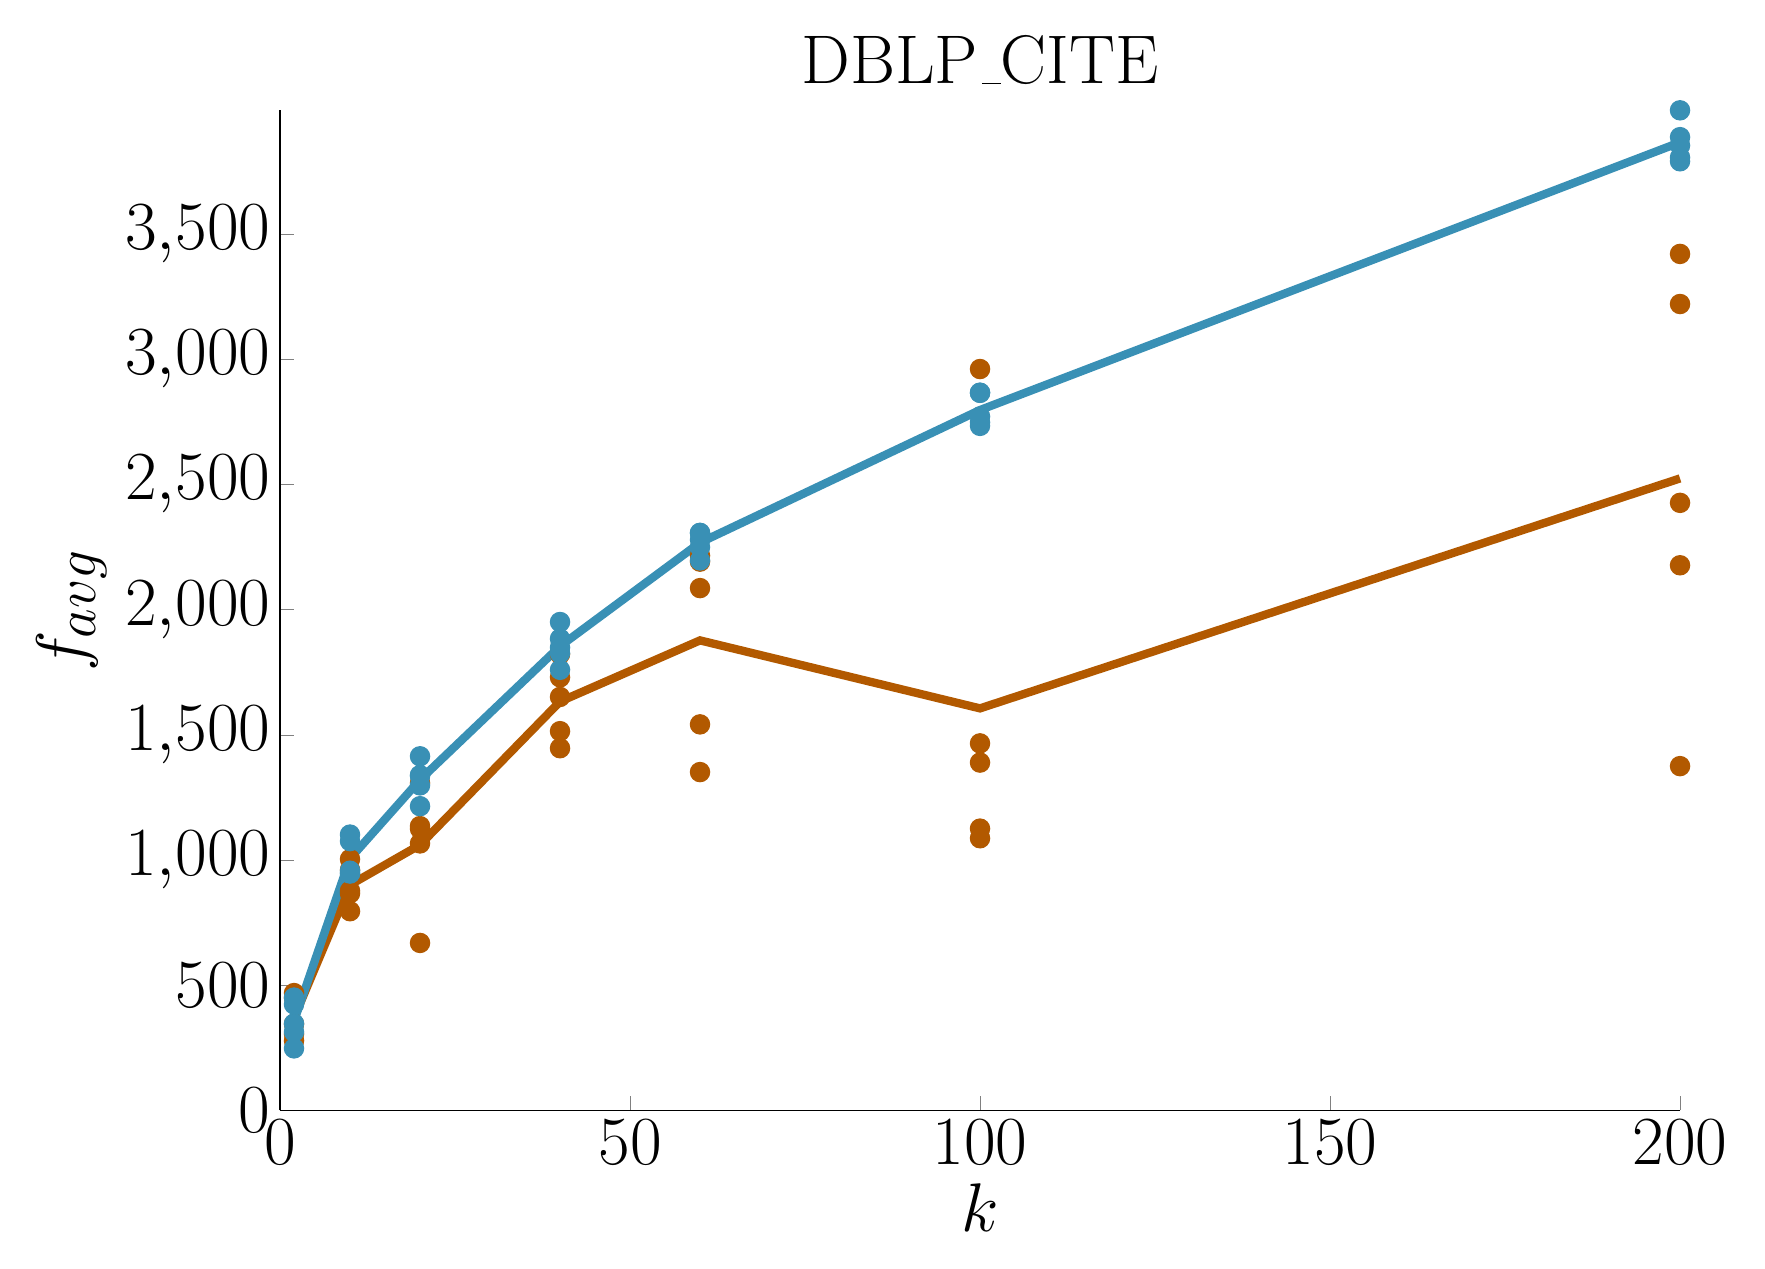
\begin{tikzpicture}

\begin{axis}[%
title style={font=\Huge},
title=DBLP\_CITE,
tick label style={font=\Huge},
label style={font=\Huge},
legend style={font=\Huge},
view={0}{90},
max space between ticks=50pt,
width=7in,
height=5in,
scale only axis,
xmin=0, xmax=200,
xtick={0, 50, 100, 150, 200},
xlabel={$k$},
ymin=0, ymax=3994.35,
%ytick={0, 200, 400, 600, 800, 1000},
ylabel={$f_{avg}$},
major tick length=5pt,
axis lines*=left,
legend cell align=left,
clip=false]

\addplot [
only marks,
mark=*,
mark size=3.5pt,
color=orange!70!black,
%solid,
%line width=2pt,
]
coordinates{
(2,277.7)(2,305.05)(2,344.8)(2,449.65)(2,468.4)(10,795.25)(10,866.5)(10,876.65)(10,959.9)(10,1003.25)(20,668.5)(20,1066.1)(20,1124.5)(20,1135.1)(20,1307.55)(40,1446.35)(40,1514.4)(40,1651.05)(40,1729.5)(40,1822.2)(60,1351.0)(60,1541.5)(60,2085.9)(60,2191.6)(60,2215.15)(100,1086.7)(100,1125.2)(100,1388.9)(100,1465.65)(100,2960.9)(200,1374.8)(200,2177.05)(200,2426.4)(200,3220.65)(200,3420.7)
};

\addplot [
only marks,
mark=*,
mark size=3.5pt,
color=cyan!70!black,
%solid,
%line width=2pt,
]
coordinates{
(2,247.4)(2,313.3)(2,346.35)(2,423.15)(2,450.4)(10,945.75)(10,947.5)(10,957.05)(10,1075.25)(10,1101.35)(20,1214.75)(20,1297.9)(20,1335.55)(20,1338.95)(20,1414.05)(40,1759.45)(40,1825.9)(40,1848.65)(40,1883.75)(40,1950.45)(60,2196.45)(60,2249.55)(60,2279.1)(60,2305.7)(60,2306.45)(100,2733.9)(100,2748.15)(100,2771.35)(100,2865.9)(100,2866.3)(200,3790.75)(200,3806.15)(200,3854.0)(200,3887.15)(200,3994.35)
};

\addplot [
color=orange!70!black,
solid,
line width=3pt
]
coordinates{
(2,369.12)(10,900.31)(20,1060.35)(40,1632.7)(60,1877.03)(100,1605.47)(200,2523.92)
};

\addplot [
color=cyan!70!black,
solid,
line width=3pt
]
coordinates{
(2,356.12)(10,1005.38)(20,1320.24)(40,1853.64)(60,2267.45)(100,2797.12)(200,3866.48)
};


\end{axis}
\end{tikzpicture}
\end{document}
